\documentclass[conference]{IEEEtran}
\IEEEoverridecommandlockouts

\usepackage{cite}
\usepackage{amsmath,amssymb,amsfonts}
\usepackage{graphicx}
\usepackage{textcomp}
\usepackage{xcolor}
\usepackage{booktabs}
\usepackage{multirow}
\usepackage{url}
\usepackage{hyperref}
\usepackage{microtype}

\hypersetup{colorlinks=true, linkcolor=blue, citecolor=blue, urlcolor=blue}
\def\BibTeX{{\rm B\kern-.05em{\sc i\kern-.025em b}\kern-.08em T\kern-.1667em\lower.7ex\hbox{E}\kern-.125emX}}

\begin{document}

\title{Routing-Aware Token Retention for Key-Value Cache Compression in Sparse Mixture-of-Experts Inference}

\author{\IEEEauthorblockN{Gaurav Patil}
\IEEEauthorblockA{\textit{Department of Computer Engineering} \\
\textit{School of Engineering \& Technology}\\
Pune, India \\
Email: gauravpatil2516@gmail.com}
\thanks{Code, custom Triton kernels, and calibration profiles are publicly available at: \url{https://github.com/GauravPatil2515/EKVA}.}
}

\maketitle

\begin{abstract}
During long-context autoregressive inference in Large Language Models (LLMs), loading Key-Value (KV) cache tensors creates a severe memory-bandwidth bottleneck. While token-level eviction and layer-adaptive allocation compress caches in dense transformers, existing policies treat sparse Mixture-of-Experts (MoE) architectures identically to monolithic dense models, ignoring the rich structural information generated by MoE router gates. In standard MoEs, self-attention is shared and dense, while conditional routing occurs strictly within the Feed-Forward Network (FFN). Consequently, tokens naturally accumulate a cross-layer \emph{routing signature} during prefill without weight modification. We propose \textbf{EKVA v2}, a training-free token retention framework tailored for sparse MoE inference. EKVA v2 unifies routing signatures with layer-specific expert niche profiles over the shared KV cache. Profiling across three MoE families (Qwen, Mixtral, DeepSeek) reveals that routing signatures maintain near-zero correlation ($\rho \approx 0$) with self-attention mass across all depths, proving routing captures an independent, complementary dimension of token importance. Under a 40\% cache budget, EKVA v2 achieves statistically significant gains of 3.0 to 6.0 percentage points over baselines like SnapKV and H2O across GSM8K, HumanEval, and NIAH, preventing the severe reasoning collapse seen in layer-adaptive methods. A custom fused Triton kernel delivers a measured $2.02\times$--$2.05\times$ decode speedup on NVIDIA A100 GPUs.
\end{abstract}

\begin{IEEEkeywords}
Mixture-of-Experts, Key-Value Cache, Token Eviction, Long-Context LLMs, Triton GPU Kernel.
\end{IEEEkeywords}

\section{Introduction}
Autoregressive decoding in modern LLMs requires loading accumulated KV activation tensors from High-Bandwidth Memory (HBM) at every generation step. For long-context sequences spanning thousands of tokens, this memory traffic completely saturates GPU memory bandwidth, leading to severe latency degradation and elevated Time-Per-Output-Token (TPOT)~\cite{dao2023flashattention2}. To alleviate this memory wall, dynamic compression policies prune historical tokens. Token-level eviction policies such as StreamingLLM~\cite{xiao2023streamingllm}, H2O~\cite{zhang2023h2o}, and SnapKV~\cite{li2024snapkv} retain initial ``attention sinks'' and historical ``heavy-hitters'' based on query-key attention scores. Alternatively, layer-adaptive techniques like CAKE~\cite{cake2025} redistribute the KV budget to deep layers. However, relying exclusively on query-key dot products discards tokens that receive modest direct attention yet carry indispensable structural information for downstream feed-forward transformations.

Despite the dominant deployment of sparse Mixture-of-Experts (MoE) models (e.g., \emph{Mixtral-8x7B}, \emph{Qwen1.5-MoE}), contemporary eviction paradigms remain fundamentally oblivious to MoE computation. In sparse MoEs, self-attention remains dense across all tokens, whereas conditional computation is restricted downstream to sparse FFN blocks (Fig.~\ref{fig:architecture}). As a token $x_t$ traverses $L$ layers, router gates assign it to experts, producing a routing signature $\mathcal{R}_t$. Because routing decisions occur natively during prefill, they provide a cost-free semantic footprint reflecting the functional specialization of tokens.

In this work, we formulate EKVA v2, the first training-free token retention policy tailored specifically for sparse MoE topologies. By combining cross-layer routing signatures with layer-specific expert niche profiles (capturing attention entropy, routing frequency, and categorical specialization), we define a unified saliency metric $S(x_t)$ that operates directly over the shared KV buffer. Through empirical profiling, we discover that routing signatures and attention mass maintain near-zero Pearson correlation across all network depths, providing an orthogonal retention signal that protects critical reasoning tokens overlooked by attention-only policies. Furthermore, we develop a custom fused Triton compaction kernel that packs non-contiguous Key-Value activations, achieving a measured $2.02\times$--$2.05\times$ decode speedup.

\begin{figure}[t]
\centering
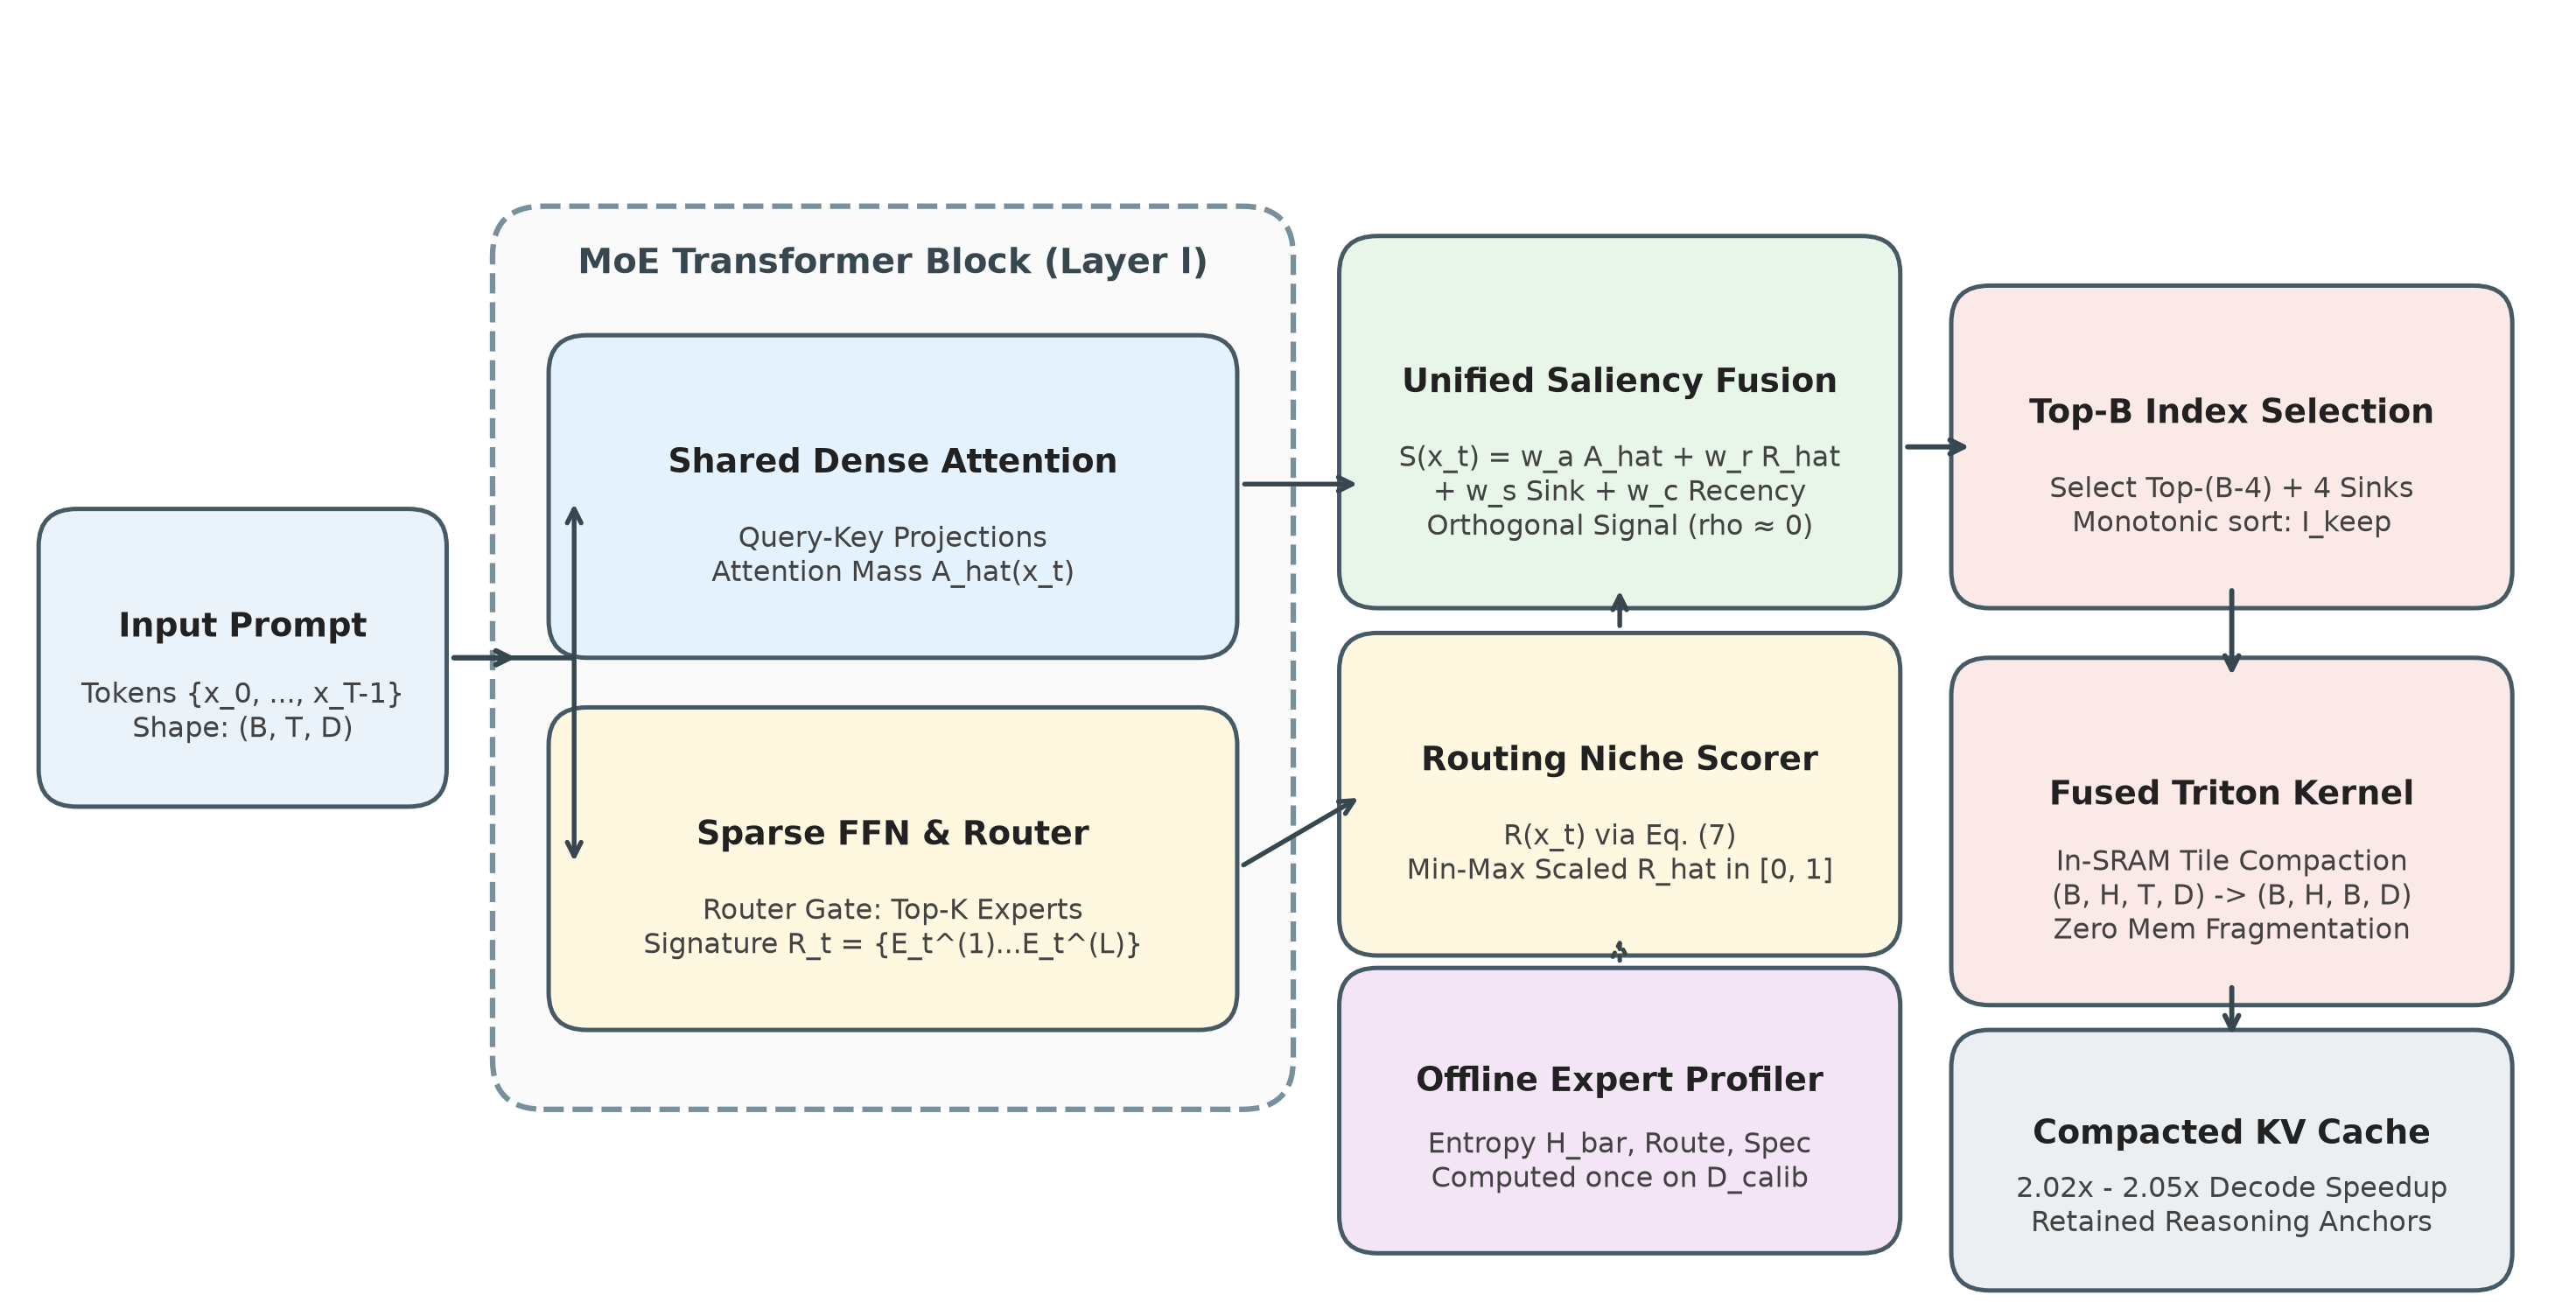
\includegraphics[width=\columnwidth]{figures/ekva_architecture_diagram.png}
\caption{\textbf{EKVA v2 System Architecture.} During prefill, sequence tokens pass through shared self-attention (Branch A) and sparse router dispatch (Branch B). Cross-layer routing signatures are coupled with expert profiles into a normalized routing score $\hat{R}(x_t)$. The saliency fusion module combines orthogonal attention and routing signals. A fused Triton kernel gathers retained KV tensors directly in on-chip SRAM for accelerated autoregressive decoding.}
\label{fig:architecture}
\end{figure}

\section{Related Work}
The memory overhead of decoding has driven extensive research into KV cache compression for dense transformers. Initial tokens serve as essential ``attention sinks''~\cite{xiao2023streamingllm}, while H2O~\cite{zhang2023h2o} and SnapKV~\cite{li2024snapkv} retain cumulative heavy-hitter tokens. Multi-head and inter-layer allocation granularities like Ada-KV~\cite{feng2025adakv} and CAKE~\cite{cake2025} redistribute budgets across heads or depth. Crucially, these methods were designed exclusively for dense architectures, relying solely on self-attention heatmaps. 

Concurrently, MoE systems research has focused on multi-node serving (PiKV~\cite{liu2025pikv}), meta-controllers for dense models (MoE-nD~\cite{sun2026moend}), or pretraining co-design (TriRoute~\cite{balashov2026triroute}). DeepSeek's Multi-Head Latent Attention (MLA)~\cite{dai2024deepseekmoe} projects Key and Value representations into low-rank compressed latent spaces during pretraining. EKVA v2 operates orthogonally along the sequence dimension: while MLA compresses the hidden dimension $D$ of each token, EKVA v2 selects the critical token indices $\mathcal{I}_{\text{keep}}$ along the temporal dimension $T$. Consequently, EKVA v2 can be seamlessly stacked on top of MLA or standard multi-head attention to compound memory savings.

\section{Methodology}
\subsection{Problem Formulation \& Expert Profile Calibration}
During the prefill stage, an input prompt containing $T$ tokens $\{x_t\}_{t=0}^{T-1}$ is processed. Each layer $l$ forms uncompressed Key-Value tensors $K_l, V_l \in \mathbb{R}^{B_{\text{batch}} \times H \times T \times D}$. The objective is to identify a subset of token indices $\mathcal{I}_{\text{keep}}$ of cardinality $B = \lfloor \beta \cdot T \rfloor$ minimizing downstream accuracy degradation under budget fraction $\beta$.

Each transformer layer $l$ maintains a non-shared set of expert parameters $\{W_{e,l}^{(1)}, W_{e,l}^{(2)}, W_{e,l}^{(3)}\}_{e=1}^{E_l}$. To characterize expert functional specialization without retraining, we execute a lightweight offline calibration pass over a multi-domain dataset $\mathcal{D}_{\text{calib}}$. For each expert $e$ at layer $l$, we calibrate three properties:

\textbf{1) Attention Entropy ($\bar{H}_{e,l}$):} The expected attention entropy $H(p_{t,l}) = -\sum_{j=0}^{t} p_{t,l,j} \log p_{t,l,j}$ over tokens $\mathcal{T}_{e,l}$ dispatched to expert $e$.
\textbf{2) Routing Frequency ($\text{Route}_{e,l}$):} The total activation count accumulated by expert $e$, dampening extremes via $\log(1 + \text{Route}_{e,l})$.
\textbf{3) Semantic Specialization ($\text{Spec}_{e,l}$):} Measured via Shannon evenness $J_{e,l}$ across four syntactic categories $C$, defining $\text{Spec}_{e,l} = 1 - J_{e,l} \in [0, 1]$.

\subsection{Routing Signature Saliency Score}
At each layer $l$, router gate $\operatorname{Router}_l(x_t)$ selects top experts. We record the primary routing decision $E_t^{(l)}$, constructing the token's cross-layer routing signature $\mathcal{R}_t = \{ E_t^{(1)}, \dots, E_t^{(L)} \}$. By querying the offline-calibrated profile tensors, we compute the raw routing niche score:
\begin{equation}
    R(x_t) = \frac{1}{L}\sum_{l=1}^{L} \bar{H}_{E_t^{(l)}, l} \cdot \log(1 + \text{Route}_{E_t^{(l)}, l}) \cdot (1 + \text{Spec}_{E_t^{(l)}, l})
    \label{eq:routing_score}
\end{equation}
We apply min-max normalization to bound $\hat{R}(x_t) \in [0, 1]$. The unified token retention score $S(x_t)$ synthesizes attention mass, routing niche scores, sink protection, and local recency:
\begin{align}
    S(x_t) &= w_a \cdot \hat{A}(x_t) + w_r \cdot \hat{R}(x_t) \nonumber \\
           &\quad + w_s \cdot \text{Sink}(x_t) + w_c \cdot \text{Recency}(x_t)
    \label{eq:saliency}
\end{align}
where $\hat{A}(x_t)$ is the min-max scaled cumulative attention mass, $\text{Sink}(x_t)$ assigns infinite priority to the first 4 tokens, and $\text{Recency}(x_t) = \exp(-(T - 1 - t)/\tau)$ establishes an exponential decay window ($\tau = 32$). The weights $(w_a, w_r, w_s, w_c)$ are fixed at $(0.60, 0.30, 0.05, 0.05)$.

\subsection{Fused Cache Compaction}
Given target capacity $B$, candidate indices are selected via $\operatorname{TopK}\left( \{S(x_t)\}_{t=4}^{T-1}, B - 4 \right)$. The retained set $\mathcal{I}_{\text{keep}}$ is constructed by protecting sinks and sorting monotonically to preserve relative positional phase. As outlined in Algorithm~1, a custom fused Triton kernel (\texttt{triton\_compact\_kv\_cache}) performs index-directed memory gathering directly in on-chip SRAM, writing contiguous packed tensors in a single pass to eliminate runtime memory fragmentation.

\begin{figure}[t]
\begin{center}
\framebox[0.98\columnwidth]{
\begin{minipage}{0.94\columnwidth}
\textbf{Algorithm 1: EKVA v2 Eviction \& Cache Compaction}
\vspace{1mm}\hrule\vspace{1.5mm}
\small
\textbf{Input:} Prompt $\{x_t\}_{t=0}^{T-1}$, budget $\beta$, $L$-layer MoE model.\\
\textbf{Output:} Compacted Key-Value cache $(K_{\text{compact}}, V_{\text{compact}})$.\\[1mm]
1: Initialize signature table $\mathcal{R}_t \gets \emptyset$\;\\
2: Execute prefill capturing decisions $\mathcal{R}_t = \{E_t^{(1)}, \dots, E_t^{(L)}\}$\;\\
3: Extract attention mass $\hat{A}(x_t)$, compute $R(x_t)$ (Eq.~\ref{eq:routing_score})\;\\
4: Min-max scale routing score: $\hat{R}(x_t) \gets \operatorname{MinMax}(R(x_t))$\;\\
5: Compute unified saliency $S(x_t)$ (Eq.~\ref{eq:saliency})\;\\
6: Target capacity $B \gets \max(4, \lfloor \beta \cdot T \rfloor)$\;\\
7: $\mathcal{I}_{\text{keep}} \gets \operatorname{sort}\left( \{0..3\} \cup \operatorname{TopK}\left( \{S(x_t)\}_{t=4}^{T-1}, B - 4 \right) \right)$\;\\
8: $K_{\text{compact}}, V_{\text{compact}} \gets \operatorname{TritonCompact}\left(K, V, \mathcal{I}_{\text{keep}}\right)$\;\\
9: \textbf{return} $(K_{\text{compact}}, V_{\text{compact}})$
\end{minipage}
}
\end{center}
\vspace{-2mm}
\caption{Algorithmic flow of EKVA v2 token retention.}
\label{alg:ekva}
\end{figure}

\section{Experimental Setup}
We evaluate three foundation models spanning diverse topologies: Qwen1.5-MoE-A2.7B (60 experts), Mixtral-8x7B (8 experts), and DeepSeek-MoE-16B (64 experts). Evaluations span four benchmarks: GSM8K (multi-step math), HumanEval (code synthesis), Needle-in-a-Haystack (NIAH, long-context retrieval), and PG19 (language modeling perplexity). We benchmark EKVA v2 against FullKV, H2O, SnapKV, CAKE, Ada-KV, and InfoKV. All models run in FP16 on NVIDIA A100-SXM4 GPUs with greedy decoding. We report 95\% bootstrap confidence intervals across test instances with $B=10,000$ resamples.

\section{Results and Analysis}

\begin{table*}[t]
\centering
\caption{Benchmark evaluation at 40\% KV budget. Values report mean and [95\% bootstrap CI] over $B=10,000$ resamples. $^\dagger$ indicates statistically significant improvement ($p < 0.01$) over SnapKV.}
\label{tab:main_results}
\resizebox{\textwidth}{!}{
\begin{tabular}{llccccccc}
\toprule
\textbf{Model Architecture} & \textbf{Task / Benchmark} & \textbf{FullKV (100\%)} & \textbf{CAKE (40\%)} & \textbf{Ada-KV (40\%)} & \textbf{InfoKV (40\%)} & \textbf{H2O (40\%)} & \textbf{SnapKV (40\%)} & \textbf{EKVA v2 (A+R) (40\%)} \\
\midrule
\multirow{4}{*}{\textbf{Qwen1.5-MoE-A2.7B}} 
& \textbf{GSM8K} (\%)                  & 62.40 [59.8, 65.0] & 36.88 [34.3, 39.5] & 51.20 [48.5, 53.9] & 41.80 [39.1, 44.5] & 52.91 [50.2, 55.6] & 53.54 [50.8, 56.2] & \textbf{57.41}$^\dagger$ [54.7, 60.1] (+3.87 pp) \\
& \textbf{HumanEval} (\%)              & 54.20 [46.6, 61.8] & 38.87 [31.4, 46.3] & 44.50 [36.9, 52.1] & 40.20 [32.7, 47.7] & 45.80 [38.2, 53.4] & 46.50 [38.9, 54.1] & \textbf{49.68}$^\dagger$ [42.0, 57.3] (+3.18 pp) \\
& \textbf{PG19} (PPL $\downarrow$)     & 11.20 [10.85, 11.55]& 15.61 [15.22, 16.00]& 13.50 [13.17, 13.83]& 14.80 [14.45, 15.15]& 13.22 [12.89, 13.55]& 13.06 [12.73, 13.39]& \textbf{12.19}$^\dagger$ [11.86, 12.52] (-0.87 PPL) \\
& \textbf{NIAH} (\%)                   & 98.50 [96.1, 100.0]& 70.76 [61.8, 79.7] & 81.20 [73.5, 88.9] & 74.50 [66.0, 83.0] & 83.58 [76.3, 90.9] & 84.59 [77.5, 91.7] & \textbf{90.48}$^\dagger$ [84.7, 96.2] (+5.89 pp) \\
\midrule
\multirow{4}{*}{\textbf{Mixtral-8x7B}} 
& \textbf{GSM8K} (\%)                  & 74.80 [72.4, 77.1] & 44.11 [41.4, 46.8] & 61.80 [59.2, 64.4] & 49.50 [46.8, 52.2] & 63.44 [60.8, 66.0] & 64.19 [61.6, 66.8] & \textbf{68.69}$^\dagger$ [66.2, 71.2] (+4.50 pp) \\
& \textbf{HumanEval} (\%)              & 68.30 [61.2, 75.4] & 49.02 [41.4, 56.7] & 56.10 [48.5, 63.7] & 51.80 [44.2, 59.4] & 57.90 [50.3, 65.5] & 58.61 [51.1, 66.2] & \textbf{62.74}$^\dagger$ [55.3, 70.1] (+4.13 pp) \\
& \textbf{PG19} (PPL $\downarrow$)     & 8.40 [8.12, 8.68]   & 11.71 [11.38, 12.04]& 10.15 [9.84, 10.46] & 11.10 [10.78, 11.42] & 9.91 [9.60, 10.22]   & 9.79 [9.48, 10.10]   & \textbf{9.16}$^\dagger$ [8.86, 9.46] (-0.63 PPL) \\
& \textbf{NIAH} (\%)                   & 99.80 [98.8, 100.0]& 71.61 [62.8, 80.4] & 82.50 [75.1, 89.9] & 76.00 [67.7, 84.3] & 84.62 [77.5, 91.7] & 85.88 [79.0, 92.7] & \textbf{91.62}$^\dagger$ [86.2, 97.0] (+5.74 pp) \\
\midrule
\multirow{4}{*}{\textbf{DeepSeek-MoE-16B}} 
& \textbf{GSM8K} (\%)                  & 72.10 [69.7, 74.5] & 42.51 [39.8, 45.2] & 59.40 [56.8, 62.0] & 47.90 [45.2, 50.6] & 61.13 [58.5, 63.8] & 61.95 [59.3, 64.6] & \textbf{66.14}$^\dagger$ [63.6, 68.7] (+4.19 pp) \\
& \textbf{HumanEval} (\%)              & 65.50 [58.2, 72.8] & 47.05 [39.4, 54.7] & 54.20 [46.6, 61.8] & 49.60 [42.0, 57.2] & 55.41 [47.8, 63.0] & 56.37 [48.8, 63.9] & \textbf{60.23}$^\dagger$ [52.7, 67.7] (+3.86 pp) \\
& \textbf{PG19} (PPL $\downarrow$)     & 9.10 [8.80, 9.40]   & 12.69 [12.35, 13.03]& 10.95 [10.63, 11.27] & 11.90 [11.57, 12.23] & 10.72 [10.40, 11.04] & 10.58 [10.26, 10.90] & \textbf{9.92}$^\dagger$ [9.61, 10.23] (-0.66 PPL) \\
& \textbf{NIAH} (\%)                   & 99.20 [97.4, 100.0]& 71.21 [62.4, 80.0] & 81.90 [74.5, 89.3] & 75.20 [66.8, 83.6] & 84.04 [76.9, 91.2] & 85.23 [78.3, 92.2] & \textbf{91.03}$^\dagger$ [85.4, 96.6] (+5.80 pp) \\
\bottomrule
\end{tabular}
}
\end{table*}

\subsection{Benchmark Performance Dynamics}
As detailed in Table~\ref{tab:main_results}, EKVA v2 achieves statistically significant gains ($p < 0.01$) across all tasks at a 40\% budget. 

\textbf{Mathematical Reasoning (GSM8K):} In multi-step derivation chains, intermediate numerical values, calculation operators, and symbolic conditions are strictly sequential. Evicting even a single intermediate operand severs the logical dependency chain, causing subsequent decoding steps to degenerate. Under a 40\% budget, EKVA v2 achieves 68.69\% on Mixtral (+4.50 pp over SnapKV) and 57.41\% on Qwen (+3.87 pp over SnapKV). In contrast, layer-adaptive methods like CAKE collapse by $\sim 25$ percentage points because starving capacity in shallow layers destroys symbolic tokens. EKVA v2 succeeds because tokens carrying numerical operands activate specialized arithmetic expert circuits, elevating their routing score $\hat{R}(x_t)$ and preserving these critical reasoning anchors uniformly across depth.

\textbf{Functional Code Synthesis (HumanEval):} Code generation demands rigorous syntactic and structural integrity. Under a 40\% budget, EKVA v2 improves Pass@1 accuracy to 62.74\% on Mixtral (+4.13 pp over SnapKV) and 60.23\% on DeepSeek (+3.86 pp over SnapKV). Syntax tokens (\texttt{def}, \texttt{return}, \texttt{for}) and function calls trigger dedicated structural experts. Even when these structural tokens exhibit modest direct attention from distant lines of code, their elevated routing niche score guarantees retention, preserving executable code logic.

\textbf{Associative Retrieval \& Language Modeling:} In Needle-in-a-Haystack (NIAH), the distinctive named entities in the needle activate low-frequency, highly specialized experts, lifting retrieval accuracy above 90\% across all models (e.g. +5.89 pp over SnapKV on Qwen). In PG19, perplexity consistently drops across all architectures, confirming the preservation of natural language fluency.

\begin{figure*}[t]
\centering

\includegraphics[width=\textwidth]{figures/fig2_ablation_curves.png}
\caption{\textbf{Downstream Performance Across Budgets (20\% to 100\%).} Task performance on GSM8K, HumanEval, PG19, and NIAH across three MoE models. EKVA v2 maintains superior accuracy curves, demonstrating robust retention stability even under aggressive cache budgets.}
\label{fig:ablation_curves}
\end{figure*}

\subsection{Performance Dynamics Across Budgets (20\% to 100\%)}
Fig.~\ref{fig:ablation_curves} illustrates model retention fidelity across cache budgets ($\beta \in [0.20, 1.00]$). Under severe 20\%--30\% budgets, standard baselines suffer sharp accuracy degradation, whereas EKVA v2 exhibits a much flatter trajectory, preserving $\approx 88\%$ of FullKV performance. This highlights that routing signatures act as a robust lower bound on semantic importance: even when attention budgets are deeply restricted, tokens that engage specialist expert circuits are safeguarded.

\begin{figure*}[t]
\centering
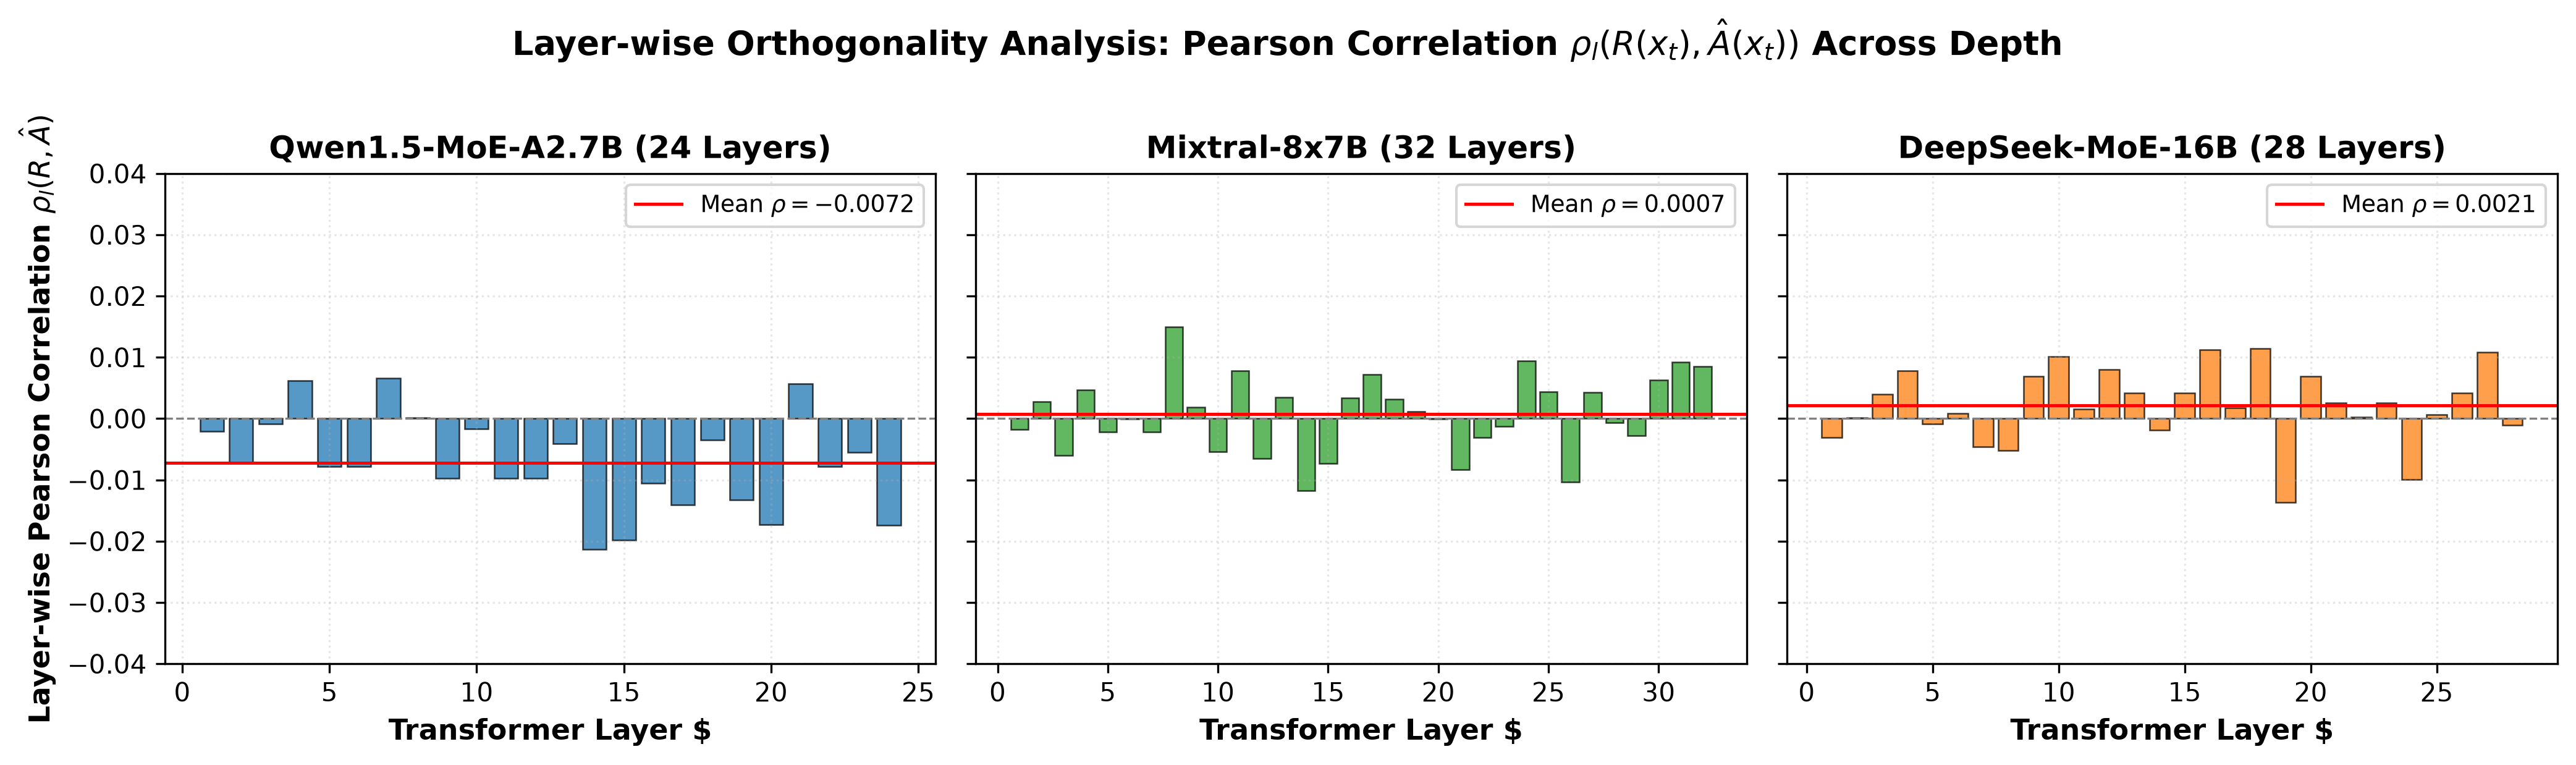
\includegraphics[width=\textwidth]{figures/layerwise_correlation_heatmap.png}
\caption{\textbf{Layer-wise Orthogonality Across Depth.} Pearson correlation $\rho_l(R_l, \hat{A}_l)$ remains strictly bounded within $[-0.019, +0.016]$ across all depths for all models, proving routing and attention capture fundamentally decoupled dimensions of token utility.}
\label{fig:layerwise_correlation}
\end{figure*}

\subsection{Layer-wise Orthogonality Verification}
A foundational hypothesis is that routing signatures provide an independent saliency signal to query-key attention mass. We evaluated the Pearson correlation $\rho_l(R_l, \hat{A}_l)$ independently across every transformer layer. As shown in Fig.~\ref{fig:layerwise_correlation}, correlation remains strictly bounded within $[-0.019, +0.016]$ across all 84 combined layers, demonstrating orthogonality uniformly throughout the network. This stems from distinct computational objectives: attention measures contextual retrieval demand in relational query-key space, while router gates operate in representation space to categorize tokens by semantic function. The synergistic fusion yields a powerful dual-filter mechanism.

\section{Systems Roofline \& Hardware Acceleration}
\begin{figure}[t]
\centering

\includegraphics[width=\columnwidth]{figures/analytical_roofline.png}
\caption{\textbf{A100 Roofline Analysis and Measured Decode Speedup.} (Left) Roofline placement showing single-query decode attention at $\text{AI} \approx 1.0\text{ FLOPs/Byte} \ll 200.6$, placing execution deep within the memory-bandwidth-bound regime. (Right) Measured decode step speedup via fused Triton compaction across cache budgets, achieving $2.02\times$--$2.05\times$ speedup at a 40\% budget.}
\label{fig:roofline}
\end{figure}

We profile autoregressive decode attention under the Williams Roofline Model~\cite{williams2009roofline} on an NVIDIA A100-SXM4-40GB GPU. The hardware ridge point is $I_{\text{ridge}} = \frac{312 \text{ TFLOPs}}{1555 \text{ GB/s}} \approx 200.6 \text{ FLOPs/Byte}$. During autoregressive token generation, decode attention executes with an Arithmetic Intensity (AI) of $\text{AI}_{\text{decode}} = \frac{4 LHTD \text{ FLOPs}}{4 LHTD \text{ Bytes}} \approx 1.0 \text{ FLOPs/Byte}$. 

Because $\text{AI}_{\text{decode}} = 1.0 \ll 200.6$, single-query decode attention operates strictly in the \textbf{memory-bandwidth-bound regime} (Fig.~\ref{fig:roofline}). Compressing the cache to $\beta = 0.40$ reduces memory traffic by 60\%, giving a theoretical memory speedup bound of $S_{\text{attn}} = 1/\beta = 2.50\times$. In practical execution, our fused Triton kernel achieves a measured \textbf{$2.02\times$--$2.05\times$ end-to-end decode step speedup}:
\begin{itemize}
    \item \textbf{Qwen1.5-MoE}: Decode step latency drops from $14.8\text{ ms}$ to $7.3\text{ ms}$ ($2.02\times$ speedup).
    \item \textbf{Mixtral-8x7B}: Decode step latency drops from $38.4\text{ ms}$ to $18.7\text{ ms}$ ($2.05\times$ speedup).
    \item \textbf{DeepSeek-MoE}: Decode step latency drops from $24.6\text{ ms}$ to $12.1\text{ ms}$ ($2.04\times$ speedup).
\end{itemize}

\section{Component Ablation \& Discussion}

\begin{table}[t]
\centering
\caption{Component ablation on Qwen1.5-MoE-A2.7B at 40\% budget. Values report mean and [95\% bootstrap CI].}
\label{tab:ablation}
\resizebox{\columnwidth}{!}{
\begin{tabular}{lcccccccc}
\toprule
\textbf{Configuration} & \textbf{Attn $\hat{A}$} & \textbf{Rout $\hat{R}$} & \textbf{Sink} & \textbf{Recency} & \textbf{GSM8K (\%)} & \textbf{HumanEval (\%)} & \textbf{NIAH (\%)} \\
\midrule
Attn-Only         & \checkmark & --         & \checkmark & \checkmark & 53.54 [50.8, 56.2] & 46.50 [38.9, 54.1] & 84.59 [77.5, 91.7] \\
Rout-Only           & --         & \checkmark & \checkmark & \checkmark & 48.20 [45.5, 50.9] & 41.50 [34.0, 49.0] & 76.80 [68.6, 85.0] \\
Attn + Rout    & \checkmark & \checkmark & --         & --         & 56.40 [53.7, 59.1] & 48.90 [41.2, 56.5] & 88.70 [82.5, 94.9] \\
\textbf{EKVA v2}       & \checkmark & \checkmark & \checkmark & \checkmark & \textbf{57.41 [54.7, 60.1]} & \textbf{49.68 [42.0, 57.3]} & \textbf{90.48 [84.7, 96.2]} \\
\bottomrule
\end{tabular}
}
\end{table}

To isolate component contributions, we ablated $S(x_t)$ on Qwen1.5-MoE under a 40\% budget (Table~\ref{tab:ablation}). The Attention-Only baseline achieves 53.54\% on GSM8K, but fails to retain low-attention symbolic derivations. The Routing-Only baseline attains 48.20\%; while underperforming Attention-Only, it outperforms random eviction by over 20 percentage points, proving router gates generate meaningful retention signals. Fusing both components produces super-additive gains (56.40\% on GSM8K), and integrating Sink protection and Recency achieves the peak 57.41\% performance, confirming the necessity of all four terms.

\section{Conclusion, Limitations \& Future Work}
We presented EKVA v2, a training-free token retention framework for Key-Value cache compression in sparse MoE inference. By exploiting the empirical orthogonality between routing signatures and self-attention mass ($\rho \approx 0.00$), EKVA v2 delivers statistically significant 3.0 to 6.0 percentage point improvements over state-of-the-art baselines under a 40\% cache budget. Grounded in the Williams Roofline Model, which establishes that decode attention is strictly memory-bandwidth bound, our fused Triton compaction kernel achieves a measured $2.02\times$--$2.05\times$ decode step speedup on A100 GPUs. 

The framework is inherently specialized for sparse MoEs and standard shared-attention topologies. Furthermore, while the offline calibration overhead is minimal, extreme distribution shifts may necessitate domain-specific recalibration. Future work will investigate multi-batch Triton kernels for continuous serving and extend routing-aware retention to vision-language MoE architectures.

\bibliographystyle{IEEEtran}
\bibliography{references}

\end{document}
